% !TeX root = ../../../wyrd.tex


\begin{WyrdSettingHeading}
    \WyrdCapLine{T}{he City of Endless Dusk} lies cradled between desert winds and ancient stars—a city of minarets and shadows, where silken veils hide sharper truths and every lantern-lit alley whispers of forgotten power.

    This is a realm of djinn and dagger, of lost empires and cursed treasures. Magic flows in stories told beneath moonlight and in the names that are never spoken aloud. Coin is king, but fate is capricious, and no pact comes without a price.

    You are a member of the House of the Crimson Falcon, a guild of shadowed repute and gilded contracts. When a noble needs a relic retrieved from a ruin no map dares name—or when a merchant prince seeks vengeance best delivered under starlight—it is your blade they call.

    Intrigue is as common as sand, and power shifts like mirage. From opulent courts to haunted catacombs, from bazaars thick with spice and secrets to the edge of the Weeping Wastes, you walk the path of the bold and the damned.

    There are treasures to claim, curses to break, and debts older than dynasties. Every contract is a story, and every story a risk. But for those who walk beneath the endless dusk, glory is never far—so long as you survive to claim it.

    Tell me, mercenary: What price would you pay to see your name etched into legend?
\end{WyrdSettingHeading}

\section{Introduction}

\textit{The City of Endless Dusk} is a setting for sword and sorcery adventures in a world inspired by tales of golden lamps, blood-stained scrolls, and forbidden gates. This chapter introduces a city built on secrets and ancient pacts, where player characters work as elite agents of the House of the Crimson Falcon—a guild for hire whose members are bound by coin, honour, and whispered reputation.

Each story is episodic—structured as a one-shot or drop-in adventure—but together they weave a deeper mythos of politics, fate, and the magic that flows just beneath the surface of civilisation. Beneath the sunless skies of the City of Endless Dusk, your players will face djinn-bound contracts, cursed artifacts, rival guilds, deadly rituals, and labyrinthine politics.

\noindent Expect:
\begin{itemize}\raggedright
    \item Tales of daring, betrayal, and arcane wonder
    \item Contracts bound in blood, secrets, and gold
    \item Encounters with djinn, spirits, and cursed relics
    \item A fluid, drop-in/drop-out format for rotating players and stories
\end{itemize}

\vspace{.75\baselineskip}\noindent
Whether your sword is sharp, your spells subtle, or your tongue golden, this chapter offers the tools to make your mark on the City—and leave a legend behind.


\begin{center}
    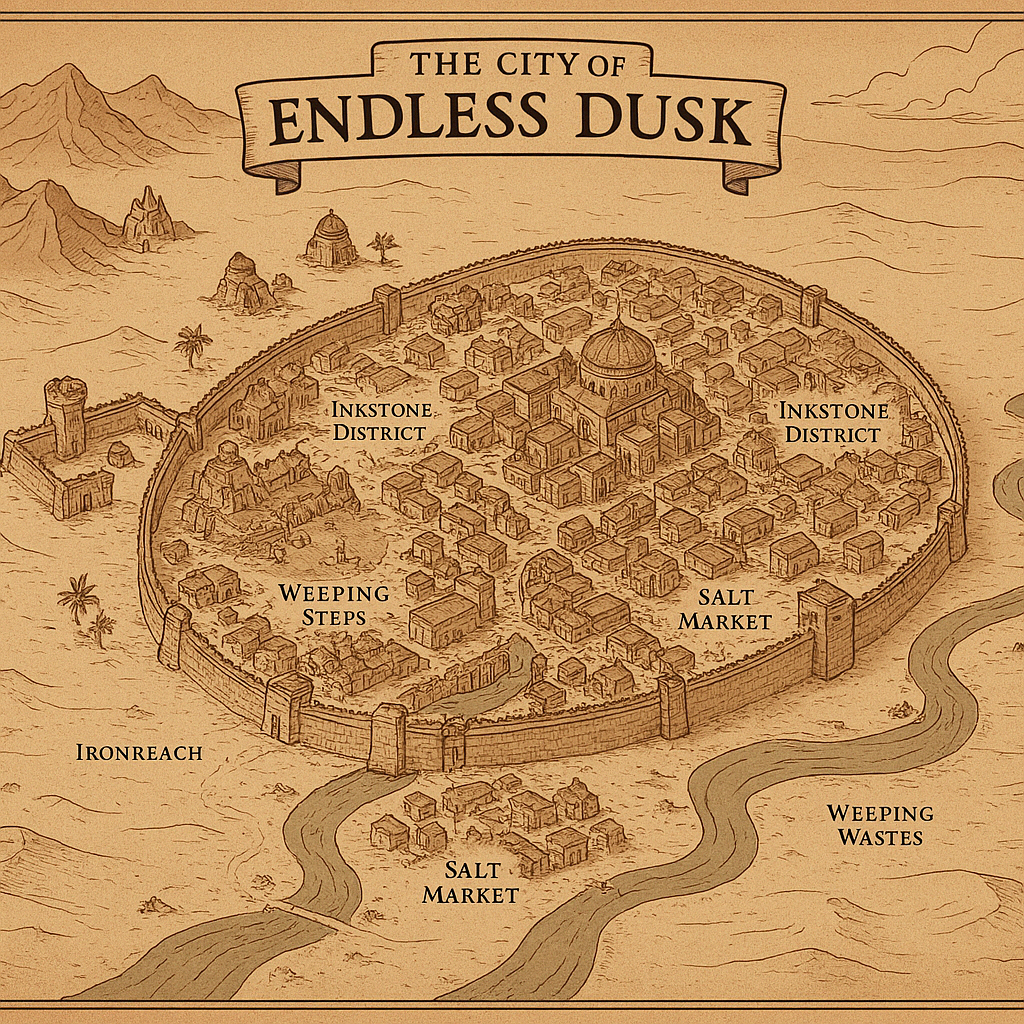
\includegraphics[width=\linewidth]{img/pageart/endless-dusk-map}
\end{center}


\section[The World of the Endless Dusk]{The World of the\\ Endless Dusk}

The City of Endless Dusk is a jewel half-buried in sand and myth. Perpetually bathed in the amber light of a sun that never fully sets, it lies on the threshold between realms—the last great haven before the desert swallows civilisation whole. Some say the city's strange twilight is a curse; others, a blessing. Most agree it is a sign: the gods still watch, and not always with mercy.

It is a place of contradictions. Marble palaces rise above crumbling ruins. Perfumed courtyards overlook shadow-choked alleys. Magi study ancient glyphs by lamplight while pickpockets pray to forgotten idols. Here, the wondrous and the wicked walk side by side—and fate has a thousand names.

The City is a nexus of trade, belief, and ambition. Its streets teem with merchants hawking silks and spices, thieves whispering secrets for sale, and holy men preaching beneath broken statues. Sorcery is feared, revered, and hidden. The old gods are silent, but their symbols remain carved in stone, waiting to be claimed by bold hands or awakened by careless ones.

The House of the Crimson Falcon serves as a central pillar of this world—a mercenary guild with a code of honour and a price for everything. When the law is bought, when the city’s rulers fear open conflict, or when something darker than steel is needed, it is the Falcons who are summoned.


\subsection{Magic and Mystery}

Magic is older than the city itself. It seeps from beneath the dunes, clings to the bones of ruined temples, and sings in the bloodlines of those who carry ancient gifts—or ancient debts. True sorcery is dangerous, rarely understood, and never free.

Most citizens know better than to speak of magic openly. Curses are real. So are the djinn—beings of smoke, fire, and broken vows. Bargains with them are sealed in soul-blood and can last generations. Yet there are always those who seek power, no matter the price.

Magic in the Endless Dusk tends to follow two paths:

\begin{itemize}
    \item \textbf{Elemental and Spirit Magic:} Drawn from the natural world, the stars, or pacts with djinn, these powers are often subtle but potent—shaping flame, calling wind, reading omens, or commanding illusions.
    \item \textbf{Relic and Rune Magic:} Artefacts, scrolls, and runes from fallen civilisations carry enchantments that still echo with power. Many are unstable or cursed, and their true effects are known only to fools or scholars with death wishes.
\end{itemize}

Those who wield magic are often marked: by glowing tattoos, strange eyes, or the scent of ozone and incense. They are respected—or feared—but never ignored.

\subsection{The City’s Many Faces}

The City of Endless Dusk is divided into countless districts, each with its own customs, factions, and dangers. Some are opulent; others are labyrinthine deathtraps. Some examples include:

\begin{itemize}\raggedright
    \item \textbf{The Pearl Quarter:} Home to nobility, embassies, and golden-domed palaces. Power here is wielded with a smile—and a dagger under the table.
    \item \textbf{The Inkstone District:} A maze of scholars, alchemists, and book-dealers. Every scroll here has a story, and some of them whisper back.
    \item \textbf{The Weeping Steps:} A haunted ruin of amphitheatres and forgotten gods. Outlaws, cultists, and cursed spirits are said to linger here.
    \item \textbf{The Salt Market:} A teeming bazaar of rare goods, rare gossip, and rarer honesty. Everything is for sale—especially you.
    \item \textbf{The Ironreach:} The edge of civilisation where relic-hunters, monster-slayers, and reckless dreamers prepare for expeditions into the Weeping Wastes beyond the city's edge.
\end{itemize}

Every district is shaped by the powers that rule it—from merchant princes to masked warlocks. Even the poorest hovel may sit above a sealed tomb, and even the grandest mansion may echo with unquiet whispers.

\subsection{Faith and Fate}

Gods are real. Or they were.

The temples remain, filled with incense and prayer, but answers are rare. Some say the gods sleep beneath the sand. Others claim they walked into the sea. Yet miracles still happen, and so do curses.

Fate is taken seriously here. Prophecies, omens, and dreams guide decisions as much as steel and coin. Many believe that every life is a thread in a vast tapestry woven by unseen hands. The Falcons learn early: deny fate, and it may come looking for you.

\textit{In the City of Endless Dusk, the line between legend and life is a breath’s width. And the sands remember everything.}

\section[Mechanics of Endless Dusk]{Mechanics of\\ Endless Dusk}

The City of Endless Dusk uses the core rules of the \textit{Wyrd Engine}, but introduces several setting-specific adjustments to better suit its sword and sorcery tone. Characters in this setting live by the blade, the bargain, or the blessing—and the system reflects those hard choices. Magic is potent but narrow in scope, and many paths lead to power—each with its own cost.

\subsection{Narrow-Scope Skills}

Unlike broader, more abstract skill lists, \textit{Endless Dusk} favours narrow-scope skills to highlight the importance of specialisation. Characters are built around what they do best—whether it’s charming a crowd, slipping through shadows, or invoking the name of a desert god to command flame.

Characters begin with the standard number of skill points, but each point purchases a specific, named skill rather than improving a general category. Sample narrow-scope skills include:
\begin{itemize}\raggedright
    \item \textbf{Sleight of Hand} — Conceal or retrieve small items unnoticed, lift purses, or swap objects in plain sight with a flick of the wrist.

    \item \textbf{Quick Draw} — Instantly ready a weapon or item in a blink, gaining the edge in moments of sudden violence or betrayal.

    \item \textbf{Track Quarry} — Follow traces left in dust, scent, or shadow, even through dense bazaars, crumbling ruins, or moonlit dunes.

    \item \textbf{Disarm Traps} — Detect and disable mechanical or magical traps, from poison-needle locks to hexed sigils guarding ancient tombs.

    \item \textbf{Persuade Nobility} — Influence the city’s elite through charm, etiquette, veiled threat, or understanding their particular pride.

    \item \textbf{Streetwise} — Navigate black markets, underworld rumours, and unspoken laws of the City’s forgotten alleys and shadow brokers.

    \item \textbf{Strike with Dagger} — Fight with precision and speed, favouring ambushes, feints, and quicksilver violence over brute strength.

    \item \textbf{Vault Obstacles} — Leap, tumble, and parkour through urban clutter or collapsed ruins—ideal for escapes, thefts, or dramatic entrances.

    \item \textbf{Arcane Lore} — Recognise runes, magical patterns, ancient glyphs, or cursed relics, and recall their legends or risks.

    \item \textbf{Summon Dust Djinn} — Call forth a minor spirit of sand and heat to perform a simple task—binding it temporarily with whispered oaths.

    \item \textbf{Mend with Light} — Channel healing through radiant energy, closing minor wounds or cleansing spiritual blight from a touched subject.

    \item \textbf{Whisper Flame} — Conjure a flickering tongue of fire in your hand, used for illumination, intimidation, or burning fragile objects.
\end{itemize}

Each of these skills operates independently, and no assumed hierarchy exists between them. Players may purchase multiple magic-related skills alongside mundane talents, reflecting the city's blurred boundary between sorcery and skill.

\subsection{Spells as Skills}

Magic in \textit{Endless Dusk} is spell-based, personal, and often perilous. Each spell is treated as a narrow-scope skill that must be purchased individually. Like other skills, spells are rated from +1 to +3—but unlike mundane abilities, casting them costs Magic Points and draws from a limited well of power.

\vspace{0.5\baselineskip}
\textbf{Spell Levels:} Each spell’s rating determines the \textbf{maximum level} it may be cast at. A spell purchased at +2 may be cast at level 1 or 2, but not 3. Each level offers a progressively stronger effect, detailed in the spell’s description.

\vspace{0.5\baselineskip}
\textbf{Magic Point Cost:} Spellcasting consumes Magic Points equal to the level cast. Casters begin with a \textbf{Magic Stress track of five points}, which recover fully between scenes unless otherwise noted. If this track is empty, casters may burn standard Fatigue or Wounds to fuel magic—at their own risk.

\vspace{0.5\baselineskip}
\textbf{DLs (Difficulty Levels):} Some spells require rolls to succeed. DLs are set by the GM and represent the target’s resistance, magical volatility, or ambient interference. DL 1 is trivial; DL 5 is formidable.

\subsubsection*{Magical Traits}

Traits may alter a caster’s ability to wield or endure magic. Some examples:

\begin{itemize}\raggedright
    \item \textbf{Djinn-Blooded (–1 Magic Point Capacity)} – Your heritage gives you powerful magic, but it burns through your soul faster. Reduce your Magic Stress track by 1.
    \item \textbf{Ritual Scholar (+1 Max Spell Rank)} – You may purchase spells at +4, though casting at this level is extremely costly and rare.
    \item \textbf{Furnace Within (+1 Magic Point Capacity)} – You have a deep well of mystical energy. Increase your Magic Stress track by 1.
    \item \textbf{Ash-Walker (–1 Cost to Ashcraft)} – Ashcraft spells cost 1 fewer Magic Point to cast (minimum 1).
\end{itemize}

\subsubsection*{Magical Schools}

Each spell belongs to a school of magic that reflects its tone, source, and cultural tradition. These schools can be used for character identity, magical relics, or determining the effects of counterspells and wards.

\vspace{0.5\baselineskip}
\textbf{Ashcraft} — The fire of ruin, rebirth, and retribution. Practiced by desert exiles, volcanic priests, and those who command flame not as heat, but as memory.

\textbf{Bloodbinding} — A sympathetic art rooted in flesh, fate, and shared essence. Used for divination, manipulation, or compulsion through the blood’s story.

\textbf{Stormcalling} — The raw invocation of sky, wind, and lightning. Stormcallers are wild emissaries of the firmament, channeling untamed forces that answer to emotion more than will.

\subsubsection*{Sample Spells}

\begin{WyrdSpell}[Ashcraft]{Breathe Ashes}
\textit{You exhale a cloud of hot, choking ash to blind and disrupt enemies. Practiced by ruin-witches and firewalkers.}
    \begin{WyrdSpellBlock}
        \item[+1] Fill a small zone (1–2 targets) with swirling ash. Targets gain a temporary penalty to sight-based actions (e.g., Aim, Notice).
        \item[+2] Obscure a wider area or multiple foes. Targets must succeed on a DL 2 check to avoid coughing fits and disorientation.
        \item[+3] Create a choking storm of embers that can blind, scatter, and burn. Foes caught within must pass a DL 3 check or suffer 1 Fatigue.
    \end{WyrdSpellBlock}
\end{WyrdSpell}

\begin{WyrdSpell}[Bloodbinding]{Echo Binding}\label{spell:echo-binding}
    \textit{Bind moments of the past into the present—allowing one to recall, relive, or even rewrite fragments of memory.}
    
    \begin{WyrdSpellBlock}
        \item[+1] Temporarily glimpse a strong memory embedded in a person, place, or object. The memory plays out as a vivid sensory illusion visible to the caster alone.
        
        \item[+2] Project the memory outward—allowing others to witness or participate in a shared memory. The caster may alter one minor detail (cosmetic only).
        
        \item[+3] Bind a memory fragment to the present, causing the past to temporarily "overlap" reality. For one scene, the environment (or people) behave as if they were still in that moment. This may include echoes of voices, spectral figures, or shifts in terrain.
    \end{WyrdSpellBlock}
\end{WyrdSpell}



\begin{WyrdSpell}[Ashcraft]{Kindle Grief}\label{spell:kindle-grief}
\textit{Ignite the sorrow of the dead, drawing out haunting fire from remembered pain.}
    \begin{WyrdSpellBlock}
        \item[+1] Create a flickering flame that weeps and whispers—useful for distraction or unsettling spirits.
        \item[+2] Force a target to relive a painful memory. DL 2 Will check or suffer a penalty to resolve-based actions.
        \item[+3] Ignite an effigy or relic to release searing emotional fire, causing Fatigue to all in range.
    \end{WyrdSpellBlock}
\end{WyrdSpell}

\begin{WyrdSpell}[Ashcraft]{Name of Dust}\label{spell:name-of-dust}
    \textit{Speak the long-forgotten name of a thing—or person—and reduce its hold on the present. The name burns away, turning history to ash.}
    
    \begin{WyrdSpellBlock}
        \item[+1] Cause a target’s name to briefly falter. For one exchange, they lose advantage from any known titles, reputation, or magical bindings tied to their identity.
        
        \item[+2] Unname an object or symbol (e.g. a ward, a sigil, a cursed relic), suppressing its magical effects for a scene. DL 2 for heavily enchanted items.
        
        \item[+3] Burn a name from memory entirely—erasing knowledge of a person, spell, or event from one target. DL 3 opposed by Will. The caster may choose whether the memory returns... or not.
    \end{WyrdSpellBlock}
\end{WyrdSpell}

\begin{WyrdSpell}[Bloodbinding]{Read the Blood}\label{spell:read-the-blood}
\textit{A drop of blood grants insight into emotions, memories, or bindings. Practitioners use ritual and taste to divine what flows beneath the skin.}
    \begin{WyrdSpellBlock}
        \item[+1] Sense the target's current emotional state and any recent intense feelings (e.g., fear, grief, joy).
        \item[+2] Glimpse surface memories from the past day or sense who the target has recently interacted with.
        \item[+3] Receive a vivid memory, hear a spoken name, or uncover spiritual tethers (e.g., blood oaths, curses). DL 3 to extract hidden or protected thoughts.
    \end{WyrdSpellBlock}
\end{WyrdSpell}

\begin{WyrdSpell}[Astral]{Lunar Lure}\label{spell:lunar-lure}
    \textit{You whisper in moonlight, drawing the mind—or body—of a target toward the phantom moon.}
    
    \begin{WyrdSpellBlock}
        \item[+1] Target becomes briefly distracted by an illusory silver glimmer. Gain +2 to Stealth, movement, or an attack against them.
        
        \item[+2] Pull a target one zone closer as they step toward the moon’s call. DL 2 Physique to resist the movement.
        
        \item[+3] Compel a creature (or weak-minded NPC) to approach the caster as if entranced by moonlight. DL 3 Will to resist; immune to damage during the approach but vulnerable afterward.
    \end{WyrdSpellBlock}
\end{WyrdSpell}

\begin{WyrdSpell}[Bloodbinding]{Blood Price}
\textit{Bind yourself to another’s fate, sharing pain and power across the tether.}
    \begin{WyrdSpellBlock}
        \item[+1] Take 1 Fatigue to grant another character +2 on their next roll. You feel their next pain in return.
        \item[+2] Link wounds—any stress or damage you take may be redirected to a bonded target. Lasts one scene.
        \item[+3] Force a bond on an unwilling foe. DL 3 Will check or they suffer 1 Fatigue whenever you do, for the rest of the scene.
    \end{WyrdSpellBlock}
\end{WyrdSpell}

\begin{WyrdSpell}[Stormcalling]{Crack the Sky}
\textit{You call down a bolt of lightning with thunderous force. Stormcallers serve no master but the wind.}
    \begin{WyrdSpellBlock}
        \item[+1] A bolt strikes a single target within sight, dealing minor damage or disruption. DL 1 to hit a moving target.
        \item[+2] The lightning arcs to an adjacent target or causes minor environmental damage (e.g., lighting oil, breaking wood). DL 2 to affect both.
        \item[+3] A storming blast strikes up to three foes or causes large-scale disruption (e.g., breaking a wall, destroying cover). DL 3 to avoid backlash.
    \end{WyrdSpellBlock}
\end{WyrdSpell}

\begin{WyrdSpell}[Astral]{Starburst Convergence}\label{spell:starburst-convergence}
    \textit{You summon a radial eruption of converging starlight, lancing out in controlled arcs.}
    
    \begin{WyrdSpellBlock}
        \item[+1] Strike one target with a focused arc of radiant force; bypasses mundane armour and knocks the target back.
        
        \item[+2] Erupt in a 10-foot burst; all creatures in the zone take 1 stress or must pass DL 2 Agility to avoid.
        
        \item[+3] Lock all enemies in the zone in a stasis field of converging beams. DL 3 Physique or be immobilised for 1 round.
    \end{WyrdSpellBlock}
\end{WyrdSpell}

\begin{WyrdSpell}[Elemental]{Lunar Flare Pulse}\label{spell:lunar-flare-pulse}
    \textit{Discharge a flash of lunar energy that sears perception and disrupts magic.}
    
    \begin{WyrdSpellBlock}
        \item[+1] Blind one target with a silver flash; they suffer –2 to their next attack or spell.
        
        \item[+2] Flare outward in a cone, blinding or disrupting the next spell cast by any creature in the area (DL 2 to resist).
        
        \item[+3] Burn out all magical effects in the zone—wards, active spells, illusions—while dealing 1 Fatigue to all spellcasters affected.
    \end{WyrdSpellBlock}
\end{WyrdSpell}

\begin{WyrdSpell}[Stormcalling]{Voice of Thunder}
\textit{Your words boom like the storm, cracking the wills of those who hear.}
    \begin{WyrdSpellBlock}
        \item[+1] Your shout echoes unnaturally. Gain +2 to Provoke or Intimidate for one roll.
        \item[+2] Stagger all enemies in a small area with a thunderclap. DL 2 Physique to remain standing.
        \item[+3] Speak a command with such force that it must be obeyed. One target must pass a DL 3 Will check or follow your short imperative.
    \end{WyrdSpellBlock}
\end{WyrdSpell}

\begin{WyrdSpell}[Elemental]{Silver Burn}\label{spell:silver-burn}
    \textit{You unleash a pulse of raw lunar fire, silvery and cold—searing flesh, faith, and memory alike.}
    
    \begin{WyrdSpellBlock}
        \item[+1] Target suffers mild radiant damage and their next magical roll takes a –1 penalty due to residual burn.
        
        \item[+2] Create a small explosion of silver fire in an area, affecting up to 3 targets. DL 2 Agility to avoid partial damage.
        
        \item[+3] Launch a streak of lunar flame that pierces magical defenses and scorches internal essence. Deals stress and temporarily suppresses one spell or magical trait for the target (GM’s choice).
    \end{WyrdSpellBlock}
\end{WyrdSpell}

\subsubsection*{Learning Magic in Play}

Spells must be purchased like other skills, but their knowledge is often hidden in ancient tomes, whispered contracts, or trials of will. Players are encouraged to roleplay the discovery of new spells—whether through stolen scrolls, bargains with djinn, or unlocking ancestral memories.

\subsubsection*{Optional Rule: Ritual Casting}

Casting a spell as a ritual (slowly, with rare components or in a sanctified space) may allow the caster to increase its level by +1 \textbf{without increasing the skill rating}, or avoid the magic point cost altogether. The GM may impose rare ingredients or complications as a tradeoff.

\begin{CommentBox}{Thematic Limits for Magic}
    The spell-as-skill model keeps magic grounded and mysterious. Magic is not a buffet of effects—it is a legacy, a language, and a risk. Let players shape their spellbooks around flavour, culture, and consequence.
\end{CommentBox}

\subsection{Skill Limits and Advancement}

Characters begin play with a total of \textbf{15 skill points} and may not start with any skill higher than \textbf{+3}. These points can be spent on mundane or magical skills in any combination, allowing for versatile and evocative builds.

\begin{itemize}\raggedright
    \item A thief with \textbf{+3 Vault Obstacles}, \textbf{+2 Steal Without Notice}, \textbf{+2 Blend into Crowds}, \textbf{+2 Quick Hands}, \textbf{+2 Feint and Strike}, \textbf{+2 Whisper Flame}, and \textbf{+2 Run Silent}.
    
    \item A swordmage with \textbf{+3 Strike with Fire}, \textbf{+3 Read the Blood}, \textbf{+2 Quick Draw}, \textbf{+2 Parry Blow}, \textbf{+2 Vault Obstacles}, and \textbf{+3 Breathe Ashes}.
\end{itemize}

This flexible structure supports a wide range of archetypes, from specialists with a narrow focus to generalists with many tools. By allowing both mundane and magical skills to draw from the same budget, the system encourages creative blends—where a fire-dancer may also be a capable duelist, or a scholar of blood may carry a hidden blade.

\subsection{Fatigue, Wounds, and Magic Costs}

The setting uses the standard \textbf{Fatigue} and \textbf{Wounds} tracks to reflect physical and mental stress. Most spell use does not automatically cost damage stress (only magic stress)—but powerful or improvised effects, particularly ritual spells, may incur Fatigue or Wounds at the GM’s discretion.

Some high-risk spell skills may include traits like:

\begin{itemize}
    \item \textbf{Fatiguing:} Using this spell always causes 1 Fatigue unless a DR check is passed.
    \item \textbf{Chaotic:} This spell has a random or unpredictable effect unless carefully prepared.
    \item \textbf{Corrupting:} Each use brings the user closer to a dark transformation, pact, or doom.
\end{itemize}

These are not mechanical “tags” in the ruleset, but rather suggested narrative prompts the GM can apply to specific spells to reinforce the dangers of magic.

\subsection{Traits and Magical Influence}

Traits in Endless Dusk can also reflect a character’s magical legacy, divine favour, or infernal pact. Examples include:

\begin{itemize}\raggedright
    \item \textbf{Djinn-Touched} – You may speak the tongue of flame and command spirits of air, fire, or shadow in limited ways, even without formal spells.
    \item \textbf{Marked by Fate} – Once per session, the GM must describe how fate intervenes subtly in your favour (or disfavours your enemies).
    \item \textbf{Breaker of Chains} – You gain a bonus when resisting magical compulsions or breaking supernatural bindings.
\end{itemize}

Traits should tie directly into the setting’s rich mythic and magical themes, and players are encouraged to write their own based on their character’s background, ancestry, or past contracts.

\subsection{Optional Rule: Spellbinding and Forgotten Words}

For groups who want a deeper spell system without departing from the core framework, the GM may permit characters to learn \textbf{Forgotten Words}: ancient incantations that function like rare, situational spells.

These are not purchased with skill points. Instead, they are discovered in play—etched on bone charms, whispered by dying spirits, or hidden in ruin-scripted vaults. Once discovered, a Forgotten Word may be used once per session or stored in a relic for repeated use.

\begin{CommentBox}{Forgotten Words as Narrative Tools}
    Forgotten Words reward exploration and risk. They work best as unique, thematic tools—such as a word that opens any door sealed in grief, or one that forces a ghost to speak the name of its killer.
\end{CommentBox}

\section{Call to Adventure}

In the \textit{City of Endless Dusk}, stories begin not with the clang of war drums—but with a whisper, a letter, a pact made beneath starless skies. Each adventure in this setting is a self-contained tale: a contract offered, a threat uncovered, or a relic desired. These stories are episodic by nature, designed for one-shots or rotating casts, yet connected by the breath of the city and the ambitions of those who walk its twilight streets.

Adventures in \textit{Endless Dusk} follow the rhythm of mercenary life—dangerous contracts, ancient secrets, fleeting alliances, and gold that disappears too quickly.

\vspace{0.5\baselineskip}
\subsection*{Structure of a Typical Job}

Most episodes begin with a summons—formal or whispered—from a faction, patron, or independent agent. Sometimes a relic needs retrieving. Other times, a caravan disappears, a tomb yawns open, or a noble house seeks to cleanse its name through silence and steel.

Each adventure usually follows this structure:

\begin{enumerate}
    \item \textbf{The Offer:} A contract or mission hook. The players are given terms, objectives, and payment—but not the full truth.
    
    \item \textbf{The Descent:} Players travel through the city or desert, navigate obstacles, uncover buried knowledge, or engage in diplomacy or subterfuge.

    \item \textbf{The Fracture:} A turning point. The job becomes more dangerous or morally fraught. Ancient powers awaken, or loyalties are tested.

    \item \textbf{The Choice:} Players must resolve the situation—by completing the job, changing its terms, or turning against those who sent them.

    \item \textbf{The Fallout:} Payment, betrayal, relics recovered, secrets exposed—or new pacts made. Each job leaves a mark.
\end{enumerate}

\vspace{0.5\baselineskip}
\subsection*{Episodic Freedom}

Each game is meant to be self-contained, so new players can drop in, and returning players can step out without derailing the overarching narrative. However, subtle continuity binds these tales: the shifting power of factions, the fate of past relics, or the recurring names whispered across episodes.

Some tools for supporting episodic continuity:

\begin{itemize}
    \item Recurring NPCs who remember what was done—and what was owed.
    \item Relics recovered in one session that resurface in another.
    \item Rumors of another group who “botched a similar job last month.”
    \item Shifting faction attitudes based on past allegiances or betrayals.
\end{itemize}

\vspace{0.5\baselineskip}
\subsection*{Who Calls?}

Jobs may come from many sources—but the most common are:

\begin{itemize}
    \item \textbf{The Sapphire Concord} — A scholarly order that hires outsiders to retrieve dangerous relics and chart ancient sites.
    \item \textbf{Merchant Houses} — Wealthy patrons in need of deniable agents to guard caravans, silence scandals, or recover stolen goods.
    \item \textbf{Faithful Orders or Cults} — Seeking sacred artifacts or protection from rivals, often with hidden motives.
    \item \textbf{Desperate Clients} — Refugees, widows, or minor nobles whose stories begin small—but often end in shadowed ruins.
\end{itemize}

\vspace{0.5\baselineskip}
\subsection*{Your Reputation Walks Ahead}

Though episodic in structure, the world remembers what you do. A group that spares a cursed creature or sells an ancient weapon may find word of it spreading. Players are encouraged to define their mercenary crew—by name, symbol, or infamy—and watch as their reputation shapes future adventures.

\begin{CommentBox}{Episodic Campaign Tips}
    Rotate missions between urban intrigue, desert survival, tomb-crawling, and magical investigation. Use recurring contracts and rival crews to build light continuity, while letting each session stand on its own. Some missions may fail—and that’s part of the tale.
\end{CommentBox}


\subimport{./}{npcs}
\subimport{./}{player-characters}


\subimport{the-nameless-moon}{the-nameless-moon}
\subimport{the-sand-remembers}{the-sand-remembers}


